\section{Sofiia Knyshoyid}
\label{sec:Sofiia_knyshoyid}

Winter landscape

\begin{figure}[htbp]
    \centering
    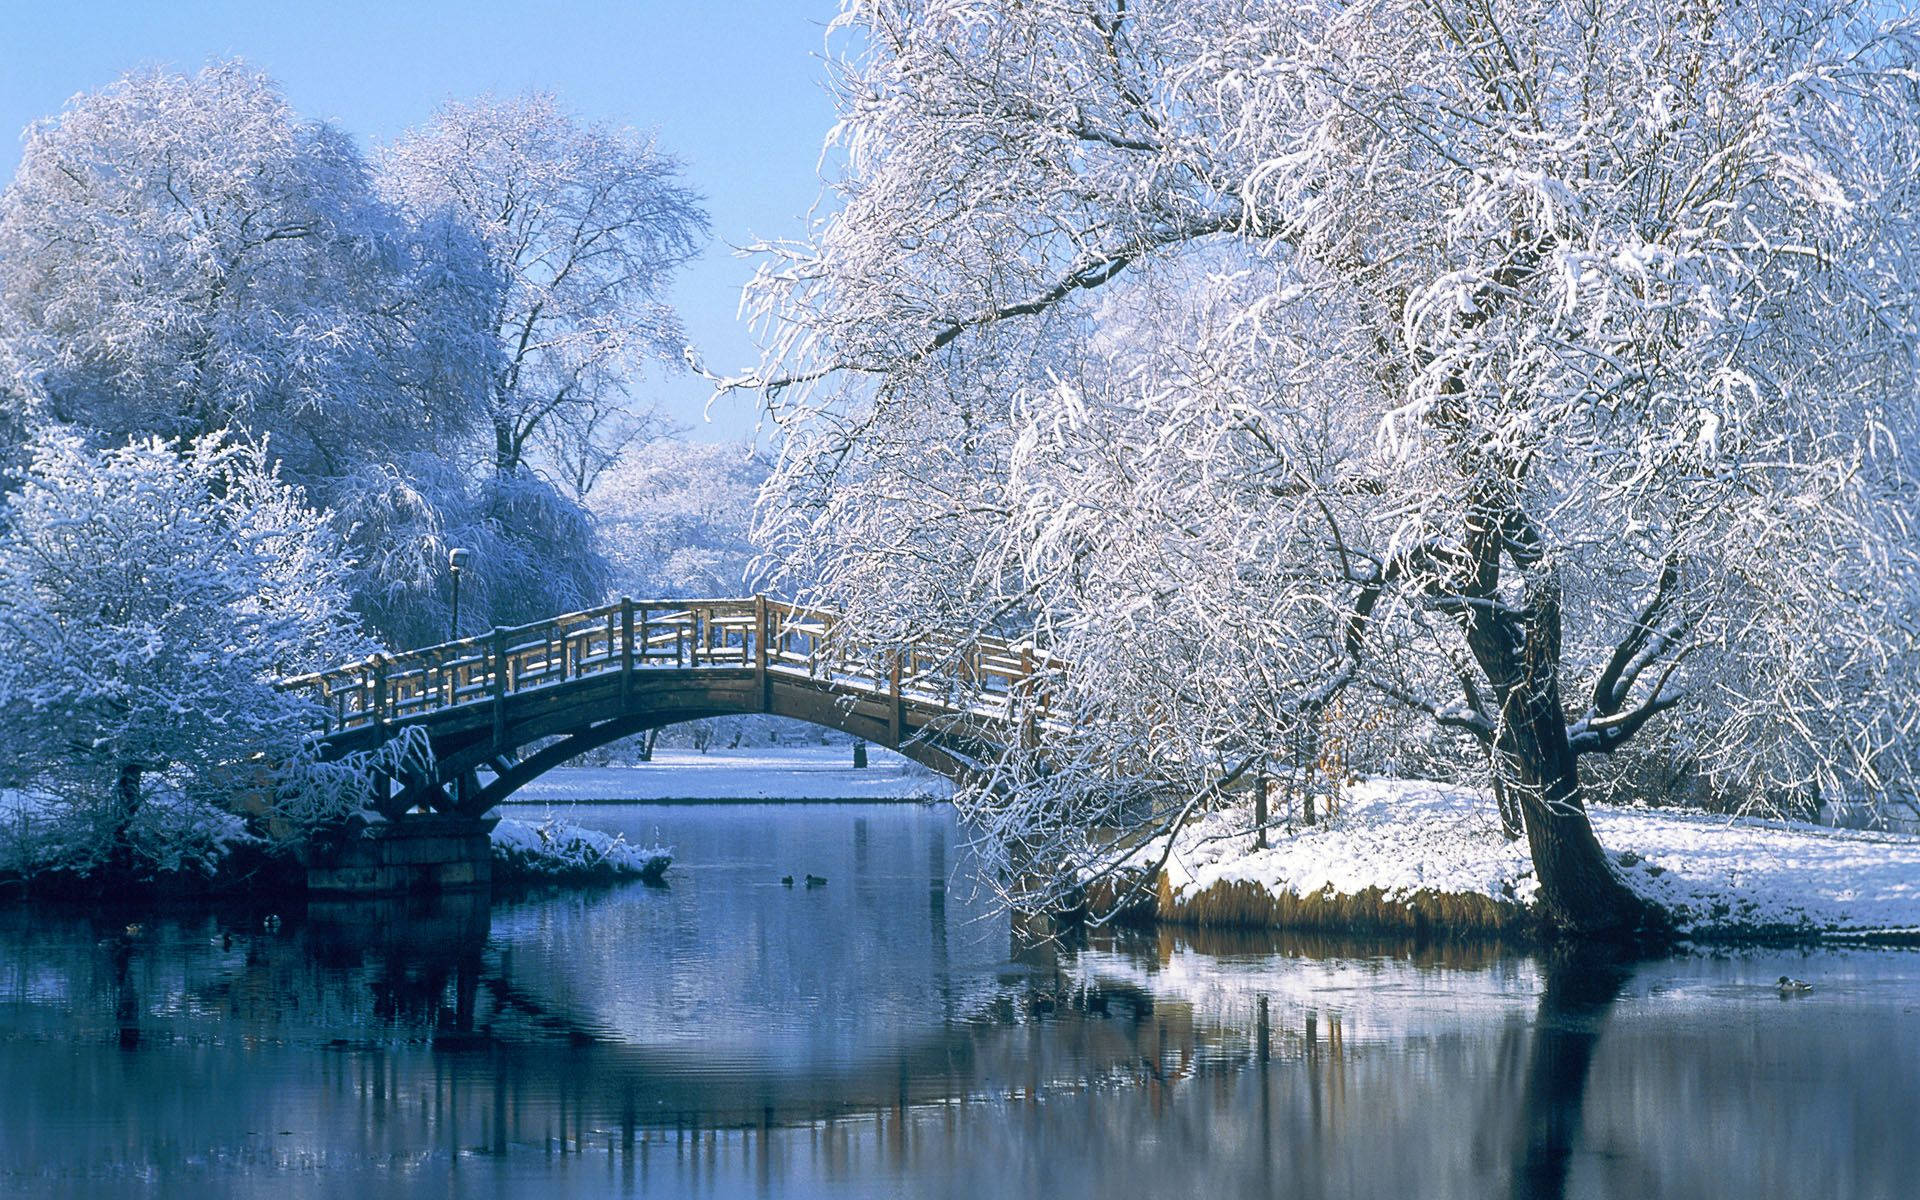
\includegraphics[width=1\textwidth]{pictures/winter_img.jpg}
    \caption{Beautiful landscape}
    \label{fig:winter}
\end{figure}

Table~\ref{sec:Sofiia_knyshoyid}, page \pageref{sec:Sofiia_knyshoyid} represents random data.
\begin{table}[htbp]
\centering
\caption{My table}
\label{My table}
\begin{tabular}{|l|l|l|l|l|l|l|}
\hline
\multicolumn{1}{|c|}{\textbf{1}} & \textbf{2} & \textbf{3} & 0 & 0 & 0 & 0 \\ \hline
\textbf{4} & \textbf{5} & \textbf{6} & 0 & 0 & 0 & 0 \\ \hline
0 & 0 & 0 & \textbf{-6} & \textbf{-5} & \textbf{-4} & \textbf{-3} \\ \hline
0 & 0 & 0 & \textbf{-3} & \textbf{-2} & \textbf{-1} & \textbf{-2} \\ \hline
\end{tabular}
\end{table}


% Dlaczego wyrażenie przeskoczyło do nowej linijki?
% Żeby nie przeskoczyło powinnaś zrobić \(...\) zamiest \[...\]
Newton’s law of universal gravitation: \(F=G*\frac{m1*m2}{r^{2}}\), which in the context of the gravity of Earth is most commonly used as:
\(F=mg\)


\newpage
\begingroup
\centering 
\section*{Info about \LaTeX{}}
\textbf{First of all,} \textbf{\LaTeX{} is a \underline{software system} \emph{for document preparation}}.  When writing, the writer uses plain text as opposed to the formatted text found in WYSIWYG word processors like Microsoft Word, LibreOffice Writer and Apple Pages. The writer uses markup tagging conventions to define the general structure of a document, to stylise text throughout a document (such as \textbf{bold} and \textit{italics}).

\noindent \textbf{What is more,} \LaTeX{}
is widely used in academia for the communication
and publication of scientific documents
in many fields.
It is easy to create tables 
in this environment \textbf{(table \ref{My table}, 
page \pageref{My table})}
or figures 
\textbf{(figure \ref{fig:winter}, page \pageref{fig:winter})}.

\endgroup
\setlength{\parindent}{30pt}



\par
\textbf{\large On the list of popular programming languages are:}
\begin{itemize}
    \item[$\heartsuit$] C/C++
    \item[$\heartsuit$] JavaScript
    \item[$\heartsuit$] Java
    \item[$\heartsuit$] Python
    \item[$\heartsuit$] R
\end{itemize}


\textbf{\large Top 3 according to some sources are:}
\begin{enumerate}
  \item Python
  \item Java
  \item JavaScript
\end{enumerate}